
Mając dany diagram splotu zorientowanego, można odwrócić jego wszystkie ogniwa albo wszystkie skrzyżowania.
Działania te nazywamy odpowiednio rewersem i~lustrem, opisujemy je w~pierwszej podsekcji.
Dalej pojawi się suma niespójna oraz spójna, odpowiednik mnożenia liczb naturalnych zbadany dokładniej przez Schuberta około 1954 roku.
\index[persons]{Schubert, Horst}%
Znacznie później (bo dopiero w~sekcji \ref{sec:tangle}) wprowadzimy jeszcze sumę i~iloczyn supłów.


\section{Lustro i~rewers. Węzły skrętne i zwierciadlane}
\begin{definition}[lustro]
% DICTIONARY;mirror;lustro/lustrzany;węzeł
\index{lustro}%
\index{węzeł!lustrzany}% TODO: to się może mylić ze zwieciadlanym
    Niech $L$ będzie zorientowanym splotem.
    Splot $\operatorname{m} L$ powstały przez odbicie splotu $L$ względem dowolnej płaszczyzny nazywamy lustrem.
\end{definition}

\begin{definition}[rewers]
% DICTIONARY;reverse;rewers/odwrotny;węzeł
\index{rewers}%
\index{węzeł!odwrotny}%
    Niech $L$ będzie zorientowanym splotem.
    Splot $\operatorname{r} L$ powstały przez odwrócenie orientacji wszystkich ogniw splotu $L$ nazywamy rewersem.
\end{definition}

\begin{comment}
{\setlength{\intextsep}{4pt plus 2pt minus 2pt}
\begin{figure}[H]
    \begin{minipage}[b]{.32\linewidth}
        \centering
        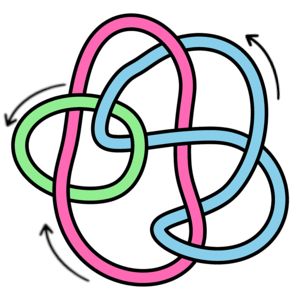
\includegraphics[height=2.2cm]{../data/links/9_3_2_mirror.png}
        \subcaption{lustro $mL$}
    \end{minipage}
    \begin{minipage}[b]{.32\linewidth}
        \centering
        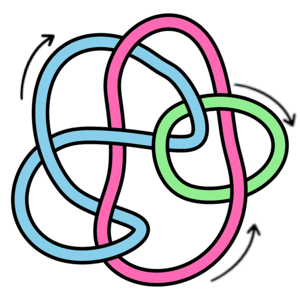
\includegraphics[height=2.2cm]{../data/links/9_3_2_base.png}
        \subcaption{przykładowy splot $L$}
    \end{minipage}
    \begin{minipage}[b]{.32\linewidth}
        \centering
        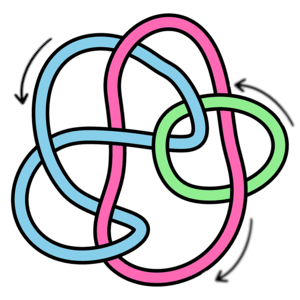
\includegraphics[height=2.2cm]{../data/links/9_3_2_reverse.png}
        \subcaption{rewers $rL$}
    \end{minipage}
\end{figure}
}
\end{comment}

Na lewym obrazku odbiliśmy diagram względem pionowej płaszczyzny, ale ten sam splot dostalibyśmy odwracając wszystkie nad- i podskrzyżowania (czyli odbijając go względem płaszczyzny papieru, ale programy graficzne nie pozwalają na wykonanie tej operacji zbyt łatwo, a~my jesteśmy trochę leniwi).

Niektórzy mówią o odbiciach lustrzanych i odwrotnościach.
Zaletą naszych oznaczeń jest to, że trudniej jest pomylić lustro z odwrotnością; ale w literaturze dominuje $L^*$ jako symbol lustra oraz $-L$ jako symbol odwrotności splotu $L$; używają ich na przykład Burde, Zieschang, Heusener \cite[s. 16]{burde2014} czy Murasugi \cite[s. 14, 24]{murasugi1996}.
Lickorish \cite[s. 4]{lickorish1997} używa $r L$ dla odwrotności oraz $\overline{L}$ dla lustra; zapewne ktoś gdzieś używa jeszcze innych znaczków.

Zauważmy, że wzięcie lustra i/lub rewersu węzła nie musi prowadzić do nowych obiektów.
Na przykład trójlistnik jest własnym rewersem: $3_1 = \operatorname{r} 3_1$, ale nie lustrem.

Dlatego wyróżniamy pięć typów symetrii splotów:

\begin{definition}[sploty zwierciadlane, odwracalne, chiralne]
% DICTIONARY;chiral;skrętny/chiralny;węzeł
% DICTIONARY;reversible;odwracalny;węzeł
% DICTIONARY;achiral/amphicheiral;zwierciadlany;węzeł
    Niech $L$ będzie splotem.
    Wtedy $L$ jest równoważny ze swoim rewersem, lustrem, rewersem lustra, wszystkimi albo żadnym z trzech wymienionych splotów;
    splot $L$ nazywamy odpowiednio:
    \begin{itemize}
        \item odwracalnym ($L = rL$),
        \item dodatnio zwierciadlanym ($L = mL$),
        \item ujemnie zwierciadlanym ($L = mrL$),
        \item całkowicie zwierciadlanym ($mL = L = rL$),
        \item całkowicie chiralnym ($mL \neq L \neq rL$).
    \end{itemize}
\index{węzeł!zwierciadlany}%
\index{węzeł!odwracalny}%
\index{węzeł!chiralny}%
\index{węzeł!skrętny|see {węzeł chiralny}}%
\end{definition}

Węzły całkowicie chiralne nazywa się czasem skrętnymi.

%    Węzły $K$, $rK$, $mK$ są parami nierównoważne. % chiral 9_32
%    Węzły $K \cong rK$ są równoważne. % reversible 3_1
%    Węzły $K \cong mrK$ są równoważne. % negative amphicheiral 8_17
%    Węzły $K \cong mK$ są równoważne. % positive amphicheiral 12a_427
%    Węzły $K, rK, mK$ są parami równoważne. % fully amphicheiral 4_1

\begin{example}
    Węzeł $9_{32}$ jest całkowicie skrętny.
\end{example}

% Całkowicie skrętne są też między innymi wszystkie węzły torusowe.
% TODO: wiki pisze Each nontrivial torus knot is prime[4] and chiral.[2]

\begin{example}
    \label{exm:trefoil_is_chiral}
    Trójlistnik jest odwracalny, ale nie zwierciadlany.
\end{example}

Przypuszczał to już Listing \cite{listing1847} w 1847 roku, ale pierwszy dowód podał dużo później, bo w 1914 roku Dehn \cite{dehn1914}. 
Oto, jak tego dokonał.
% równik = equator
% równoleżnik = parallel (of latitude), najdłuższy równoleżnik to równik
% południk = meridian (of longitude)
% TODO: meridian pojawia się u Burdego, Zieschanga na s. 21 (2013) (numeracja papierowa)
% TODO: naprostować bałagan z meridian/longitude w całej książce
% https://math.stackexchange.com/questions/2511364/how-did-dehn-prove-that-the-trefoil-is-chiral myli te pojęcia: pisze o meridian i longitude, kiedy oryginalna praca Dehna operowała na longitude i latitude
\begin{proof}[Niedowód]
    Iloraz grafu Cayleya dla grupy podstawowej trójlistnika, $G = \pi_1(S^3 - K)$, zanurza się w~produkt $\mathbb H^2 \times \R$, co pozwala wyznaczyć grupę zewnętrznych automorfizmów grupy $G$, $\Z/2\Z$.
\index{grupa!podstawowa}
% DICTIONARY;latitude;szerokość geograficzna;geografia
% DICTIONARY;longitude;długość geograficzna;geografia
% DICTIONARY;meridian (of longitude);południk;geografia
% DICTIONARY;parallel (of latitude);równoleżnik;geografia
% DICTIONARY;---;geografia;-
Korzystając z~południków i~równoleżników pokazał następnie, że nietrywialny automorfizm zewnętrzny odwraca orientację przestrzeni otaczającej.
\end{proof}

My przekonamy się o~tym po wyznaczeniu wielomianu Jonesa trójlistnika (wniosek \ref{cor:jones_of_amphicheiral}).
Burde, Zieschang, Heusener \cite[s. 79]{burde2014} wyprowadzają ten sam wynik z~własności węzłów rozwłóknionych.

\begin{example}
    Węzeł $8_{17}$ jest zwierciadlany ujemnie, ale nie odwracalny.
\end{example}

Nieodwracalności $8_{17}$ dowiedli niezależnie około 1979 roku Kawauchi \cite{kawauchi1979} oraz Bonahon, Siebenmann \cite{bonahonf1979}.

Sześćdziesiąt lat temu matematycy nie byli pewni, czy węzły nieodwracalne w~ogóle istnieją \cite[problem 10]{fox1962};
obecnie wiadomo, że nieodwracalne są prawie wszystkie węzły (Murasugi \cite[s.~46]{murasugi1996}).
\index[persons]{Murasugi, Kunio}%
W~roku 1962 Ralph Fox wskazał kilku kandydatów do tego tytułu.
\index[persons]{Fox, Ralph}%
Hale Trotter odkrył rok później nieskończoną rodzinę nieodwracalnych precli, patrz \ref{prp:pretzel_not_invertible}.
\index[persons]{Trotter, Hale}%

% MAKOTO SAKUMA - A SURVEY OF THE IMPACT OF THURSTON’S WORK ON KNOT THEORY
% Hartley [129] realized that one can apply this method to the problem of identifying noninvertible knots, as follows. Suppose no automorphism of Γ maps γ to γ−1. Then the set R(G(K), Γ, γ) is possibly different from the set R(G(K), Γ, γ−1), and there is a chance to show noninvertibility of K by comparing the homology invariants associated with φ ∈ R(G(K), Γ, γ) with those associated with φ′ ∈ R(G(K), Γ, γ−1). Hartley showed that this method is quite effective: he completely determined the 36 non-invertible knots up to 10 crossings claimed by Conway to be noninvertible.

\begin{example}
    Węzeł $12a_{427}$ jest zwierciadlany dodatnio, ale nie odwracalny.
\end{example}

Żaden inny węzeł pierwszy o mniej niż 13 skrzyżowaniach nie ma tej cechy.

\begin{example}
\label{property_of_eight_knot}%
    Ósemka $4_1$ jest całkowicie zwierciadlana.
\end{example}

To najprostszy typ symetrii, wystarczy jawnie wskazać przekształcenie między diagramem węzła, jego lustra oraz odwrotności.

\label{con:tait_fourth}%
Tait odnosił wrażenie, że zwierciadlane węzły mają parzysty indeks skrzyżowań, ale Hoste, Thistlethwaite znaleźli w~1998 kontrprzykład o~piętnastu skrzyżowaniach, $15_{700}$. % wg https://mathworld.wolfram.com/AmphichiralKnot.html
(Czwarta) hipoteza Taita jest prawdziwa dla węzłów pierwszych, alternujących.
\index{hipoteza!Taita}%

Poniższa tabela oparta jest (kolejno) o~ciągi
\href{https://oeis.org/A051766}{51766},
\href{https://oeis.org/A051769}{51769},
\href{https://oeis.org/A051768}{51768},
\href{https://oeis.org/A051767}{51767},
\href{https://oeis.org/A052400}{52400},
z bazy danych ``The On-Line Encyclopedia of Integer Sequences'' (OEIS).

\begin{table}[h]
    \centering
    \begin{tabular}{@{}*{20}l@{}} \toprule
        skrzyżowania & 3 & 4 & 5 & 6 & 7 & 8 & 9 & 10 & 11 & 12 & 13 & 14 \\ \midrule
        całkowicie skrętne & 0 & 0 & 0 & 0 & 0 & 0 & 2 & 27 & 187 & 1103 & 6919 & 37885 \\
        odwracalne & 1 & 0 & 2 & 2 & 7 & 16 & 47 & 125 & 365 & 1015 & 3069 & 8813 \\
        $-$ zwierciadlane & 0 & 0 & 0 & 0 & 0 & 1 & 0 & 6 & 0 & 40 & 0 & 227 \\
        $+$ zwierciadlane & 0 & 0 & 0 & 0 & 0 & 0 & 0 & 0 & 0 & 1 & 0 & 6 \\
        zwierciadlane & 0 & 1 & 0 & 1 & 0 & 4 & 0 & 7 & 0 & 17 & 0 & 41 \\
        \bottomrule
        \hline
    \end{tabular}
    \caption{Liczba węzłów pierwszych o~poszczególnych typach symetrii}
\end{table}

\begin{definition}
    Niech $K \subseteq S^3$ będzie węzłem.
    Jeśli istnieje inwolucja pary $(S^3, K)$, która zachowuje orientację sfery, ale odwraca orientację węzła, to węzeł $K$ nazywamy silnie odwracalnym.
\end{definition}

To jest definicja 10.3.2 z monografii Kawauchiego \cite{kawauchi1996}.

\begin{proposition}
    Jeśli węzeł jest silnie odwracalny, to jest też odwracalny.
\end{proposition}

Hipotezę, że każdy odwracalny węzeł jest też silnie odwracalny, postawił Montesinos \cite[problem 1.6]{kirby1978}, on też zdefiniował klasę silnie odwracalnych węzłów \cite{montesinos1975}.
\index[persons]{Montesinos, José}%
Jednakże...

\begin{proposition}
    Istnieją odwracalne węzły, które nie są silnie odwracalne.
\end{proposition}

\begin{proof}
\index[persons]{Hartley, Richard}%
\index[persons]{Whitten, Wilbur}%
    Stosowne przykłady podali niezależnie od siebie Hartley \cite[s. 183]{hartley1980} oraz Whitten \cite{whitten1981} (węzeł $K$ jest silnie odwracalny wtedy i tylko wtedy, gdy każdy jego dubel jest silnie nieodwracalny, wynika stąd, że pewien dubel $8_{17}$ nie jest silnie odwracalny; jednocześnie Schubert \cite[s. 235]{schubert1953} pokazał, że duble są odwracalne).
\end{proof}

Ale hiperboliczny węzeł odwracalny jest silnie odwracalny, wspomina o tym bez dowodu Kawauchi.

\begin{proposition}
    Każdy wielomian Alexandera jest realizowany przez pewien silnie odwracalny węzeł.
\end{proposition}

\begin{proof}[Niedowód]
\index[persons]{Sakai, Tsuyoshi}%
    Sakai \cite{sakai1983} dla każdego cyklicznego modułu Alexandera $M$ skonstruował silnie odwracalny węzeł $K$, którego modułem Alexandera jest właśnie $M$.
\end{proof}

% Koniec podsekcji Lustro i rewers




\subsection{Węzły okresowe}
\index{węzeł!okresowy|(}%
Można wyróżnić jeszcze jeden rodzaj symetrii.

% DICTIONARY;period;okres;-
% DICTIONARY;periodic;okresowy;węzeł
\begin{definition}
\label{def:period}%
    Węzeł $K$ nazywamy $n$-okresowym, jeśli istnieje obrót $f \colon \R^3 \to \R^3$ o~kąt $2\pi/n$ wokół pewnej prostej $l$, rozłącznej z~węzłem $K$, taki że $f(K) = K$.
\end{definition}

Zamiast obrotów można rozpatrywać dowolne odwzorowania okresowe $f \colon S^3 \to S^3$, których zbiór punktów stałych jest rozłączny z węzłem $K$, homeomorficzny z $S^1$ oraz które trzymają węzeł $K$ w miejscu, ale dostaje się wtedy dokładnie taką samą klasę węzłów.
Czemu?
Wynika to z hipotezy Smitha, otrzymanej z połączenia głębokich teorii dotyczących geometrii i topologii 3-rozmaitości.
\index{hipoteza!Smitha}%
Kawauchi \cite[s. 125]{kawauchi1996} odsyła tu do książki Morgana, Bassa \cite{morgan1984}, gdzie znajdziemy problem, jego historię i rozwiązanie.
\index[persons]{Morgan, John}%
\index[persons]{Bass, Hyman}%

\begin{proposition}
    Zbiór wszystkich okresów jest niezmiennikiem węzłów.
\end{proposition}

Nieodwracalny węzeł $8_{17}$ nie posiada żadnych okresów.
% ćwiczenie 10.1.5 w Kawauchi
Węzeł $5_1$ jest 5-okresowy, co widać na standardowym diagramie, oraz 2-okresowy, tę drugą symetrię można dostrzec na diagramie realizującym liczbę mostową.
Trójlistnik ma dokładnie dwa okresy, $2$ i~$3$.
Ogólniej, jak głosi Kawauchi \cite[ćwiczenie 10.1.9]{kawauchi1996}:

\begin{proposition}
    Jedynymi okresami węzła $(p, q)$-torusowego są dzielniki liczb $p$ oraz $q$.
\end{proposition}

Murasugi podał dwa warunki, które musi spełniać węzeł o~okresie $n = p^r$, gdzie $r$ jest liczbą pierwszą.
Do ich zrozumienia potrzebujemy dwóch definicji.

\begin{definition}
    Niech $f$ będzie obrotem z definicji \ref{def:period}, zaś $p \colon \R^3 \to \R^3/f \simeq \R^3$ rzutem na przestrzeń ilorazową.
% DICTIONARY;quotient;ilorazowy;węzeł
\index{węzeł!ilorazowy}%
    Wtedy $p(K)$ nazywamy \emph{węzłem ilorazowym}, zaś $K$ to jego $n$-krotne nakrycie.    
\end{definition}

Ładny rysunek węzła ilorazowego znaleźliśmy u Kawauchiego \cite[s. 122]{kawauchi1996}.

\begin{definition}
    Niech $K$ będzie zorientowanym węzłem, zaś $l$ zorientowaną półprostą, która nie jest styczna do węzła $K$.
    Wtedy różnicę między liczbą skrzyżowań dodatnich oraz ujemnych wzdłuż półprostej (bez znaku) nazywamy indeksem zaczepienia $\lambda$ węzła $p(K)$.
\end{definition}

\begin{proposition}[warunek Murasugiego]
\index{warunek!Murasugiego}%
\label{prp:murasugi_periodic}%
    Niech $K$ będzie węzłem o~okresie $n = p^r$, gdzie $p$ jest liczbą pierwszą.
    Niech $J$ będzie jego węzłem ilorazowym, z~indeksem zaczepienia $\lambda$.
    Wtedy wielomian $\alexander_J$ jest dzielnikiem wielomianu $\alexander_K$ oraz istnieje pewna całkowita liczba $k$, taka że
    \begin{equation}
        \alexander_K(t) \equiv \pm t^k \alexander_J(n)^n \left(1 + t + t^2 + \ldots + t^{\lambda - 1}\right)^{n-1} \mod p.
    \end{equation}
\end{proposition}

\begin{proof}[Niedowód]
    Mozolne operacje na macierzach, których wyznacznikiem jest wielomian Alexandera, patrz \cite{murasugi1971}.
    Kawauchi przedstawia inny dowód: najpierw dowodzi tego dla węzła torusowego $T_{n, d}$, którego węzłem ilorazowym jest niewęzeł.
    W ogólnym przypadku, korzysta z relacji kłębiastej dla wielomianu Conwaya.
    Szczegóły oraz odsyłacze do dalszych prac znaleźć można w jego przeglądowej publikacji \cite[s. 122-124]{kawauchi1996}.
\end{proof}

Z prac Borodzika (m.in. \cite{grabowski20} napisanej z Grabowskim, Królem i Marchwicką) dowiedzieliśmy się, że podany wyżej warunek Murasugiego jest tylko jednym z wielu ograniczeń, jakie musi spełniać węzeł okresowy.
Autorzy wymieniają:
\begin{itemize}
    \item warunek Murasugiego udoskonalony przez Davisa, Livingstona \cite{davis1991},
\index[persons]{Davis, James}%
\index[persons]{Livingston, Charles}%
    \item kryterium Naika z homologiami rozgałęzionego nakrycia \cite{naik1997},
\index[persons]{Naik, Swatee}%
\index{homologie}%
\index{rozgałęzione nakrycie}%
    \item kryterium Traczyka z wielomianem Jonesa \cite{traczyk1991},
\index{wielomian Jonesa}%
\index[persons]{Traczyk, Paweł}%
    \item kryterium Przytyckiego z wielomianem HOMFLY-PT \cite{przytyckij1989},
\index{wielomian HOMFLY-PT}%
\index[persons]{Przytycki, Józef}%
    \item kryterium Naika z niezmiennikiem Cassona-Gordona,
\index{niezmiennik Cassona-Gordona}%
\index[persons]{Naik, Swatee}%
    \item kryterium Hillmana, Livingstona, Naika ze skręconym wielomianem Alexandera \cite{hillman2006},
\index{wielomian Alexandera!skręcony}%
\index[persons]{Hillman, Jonathan}%
\index[persons]{Livingston, Charles}%
\index[persons]{Naik, Swatee}%
    \item kryterium Jabuki, Naika z homologią Floera \cite{jabuka2016},
\index{homologia Floera}%
\index[persons]{Jabuka, Stanisław}%
\index[persons]{Naik, Swatee}%
    \item kryteria Borodzika, Politarczyka z homologią Chowanowa, \cite{politarczyk2017}, \cite{politarczyk2021},
\index{homologia Chowanowa}%
\index[persons]{Borodzik, Maciej}%
\index[persons]{Politarczyk, Wojciech}%
    \item kryterium Chena z grupą podstawową \cite{chen2018}.
\index{grupa podstawowa}%
\index[persons]{Chen, Haimiao}%
\end{itemize}
% Sakumy nie ma, bo nie został wymieniony ze słowem criterion; być może napisał coś ogólnego? 
\index{kryterium Naika (okresowości)}%

\index{węzeł!okresowy|)}%

% koniec podsekcji Węzły okresowe




\subsection{Suma niespójna i~suma spójna}

\begin{definition}[suma niespójna]
% DICTIONARY;distant union;suma niespójna;-
\index{suma niespójna}%
    Niech $L_1$ oraz $L_2$ będą splotami, które leżą po różnych stronach ustalonej płaszczyzny w przestrzeni $\R^3$.
    Teoriomnogościową sumę $L_1 \sqcup L_2$ nazywamy sumą niespójną splotów $L_1$ i $L_2$.
\end{definition}

\begin{definition}[suma spójna]
% DICTIONARY;connected sum;suma spójna;-
\index{suma spójna}%
\label{def:connected_sum}%
    Niech $K_1, K_2$ będą zorientowanymi węzłami.
    Natnijmy każdy z nich w dwóch punktach tego samego krótkiego łuku, a następnie zszyjmy dwoma łukami, które nie przecinają już istniejących, jak na obrazku.
    Otrzymany węzeł nazywamy sumą spójną węzłów $K_1$ oraz $K_2$ i oznaczamy przez $K_1 \shrap K_2$.
\begin{comment}
    \[
        \begin{tikzpicture}[baseline=-0.65ex,scale=0.09]
        \useasboundingbox (-12, -15) rectangle (12, 10);
        \begin{knot}[clip width=5, flip crossing/.list={5}, ignore endpoint intersections=false,]
            \strand[thick] (-3.5, -3.5) [in=down, out=up] to (3.5, 3.5);
            \strand[thick] (3.5, 3.5) [in=right, out=up] to (-4.5, 10);
            \strand[thick] (-4.5, 10) [in=up, out=left] to (-10, 3.5);
            \strand[thick] (-10, 3.5) to (-10, -3.5);
            \strand[thick] (-10, -3.5) [in=left, out=down] to (-4.5, -10);
            \strand[thick] (-4.5, -10) [in=down, out=right] to (3.5, -3.5);
            \strand[thick] (3.5, -3.5) [in=down, out=up] to (-3.5, 3.5);
            \strand[thick] (-3.5, 3.5) [in=left, out=up] to (4.5, 10);
            \strand[thick] (4.5, 10) [in=up, out=right] to (10, 3.5);
            \strand[thick, -Latex] (10, 3.5) to (10, -3.5);
            \strand[thick] (10, -3.5) [in=right, out=down] to (4.5, -10);
            \strand[thick] (4.5, -10) [in=down, out=left] to (-3.5, -3.5);
            \node at (0, -15) {$K_1$};
        \end{knot}
        \end{tikzpicture}
        \shrap
        \begin{tikzpicture}[baseline=-0.65ex,scale=0.09]
        \useasboundingbox (-12, -15) rectangle (12, 10);
        \begin{knot}[clip width=5, flip crossing/.list={6}, ignore endpoint intersections=false,]
            \strand[thick] (-3.5, -3.5) [in=down, out=up] to (3.5, 3.5);
            %\strand[thick] (3.5, 3.5) [in=right, out=up] to (-4.5, 10);
            %\strand[thick] (-4.5, 10) [in=up, out=left] to (-10, 3.5);
            \strand[thick] (-10, -3.5) [in=left, out=up] to (0, 6.5);
            \strand[thick, Latex-] (-10, -3.5) [in=left, out=down] to (-4.5, -10);
            \strand[thick] (-4.5, -10) [in=down, out=right] to (3.5, -3.5);
            \strand[thick] (3.5, -3.5) [in=down, out=up] to (-3.5, 3.5);
            %\strand[thick] (-3.5, 3.5) [in=left, out=up] to (4.5, 10);
            %\strand[thick] (4.5, 10) [in=up, out=right] to (10, 3.5);
            \strand[thick] (10, -3.5) [in=right, out=up] to (0, 6.5);
            \strand[thick] (10, -3.5) [in=right, out=down] to (4.5, -10);
            \strand[thick] (4.5, -10) [in=down, out=left] to (-3.5, -3.5);
            %
            \strand[thick] (-3.5, 3.5) [in=left, out=up] to (0, 10);
            \strand[thick] (3.5, 3.5) [in=right, out=up] to (0, 10);
            \node at (0, -15) {$K_2$};
        \end{knot}
        \end{tikzpicture}
        =
        \begin{tikzpicture}[baseline=-0.65ex,scale=0.09]
        \useasboundingbox (-27, -15) rectangle (27, 10);
        \begin{knot}[clip width=5, flip crossing/.list={5, 22, 23}, ignore endpoint intersections=false,]
            \strand[thick] (-18.5, -3.5) [in=down, out=up] to (-11.5, 3.5);
            \strand[thick] (-11.5, 3.5) [in=right, out=up] to (-19.5, 10);
            \strand[thick] (-19.5, 10) [in=up, out=left] to (-25, 3.5);
            \strand[thick] (-25, 3.5) to (-25, -3.5);
            \strand[thick] (-25, -3.5) [in=left, out=down] to (-19.5, -10);
            \strand[thick] (-19.5, -10) [in=down, out=right] to (-11.5, -3.5);
            \strand[thick] (-11.5, -3.5) [in=down, out=up] to (-18.5, 3.5);
            \strand[thick] (-18.5, 3.5) [in=left, out=up] to (-10.5, 10);
            \strand[thick] (-10.5, 10) [in=left, out=right] to (-5, 2);
            \strand[thick, -Latex] (-5, 2) to (-5+6, 2);
            \strand[thick] (5, 2) to (-5+6, 2);
            \strand[thick] (3, -2) to [in=left, out=right] (10.5, -10);
            \strand[thick, -Latex] (3, -2) to (-3, -2);
            \strand[thick] (-5, -2) to (-3, -2);
            \strand[thick] (-5, -2) [in=right, out=left] to (-10.5, -10);
            \strand[thick] (-10.5, -10) [in=down, out=left] to (-18.5, -3.5);
            %%%
            \strand[thick] (11.5, -3.5) [in=down, out=up] to (18.5, 3.5);
            \strand[thick] (-10 +15, 2) [in=left, out=right] to (15, 6.5);
            \strand[thick] (10.5, -10) [in=down, out=right] to (18.5, -3.5);
            \strand[thick] (18.5, -3.5) [in=down, out=up] to (11.5, 3.5);
            \strand[thick] (25, -3.5) [in=right, out=up] to (15, 6.5);
            \strand[thick] (25, -3.5) [in=right, out=down] to (19.5, -10);
            \strand[thick] (19.5, -10) [in=down, out=left] to (11.5, -3.5);
            \strand[thick] (11.5, 3.5) [in=left, out=up] to (15, 10);
            \strand[thick] (18.5, 3.5) [in=right, out=up] to (15, 10);
            %%%
            \node at (0, -15) {$K_1 \shrap K_2$};
        \end{knot}
        \end{tikzpicture}
    \]
\end{comment}
\end{definition}

W topologii rozważa się podobną operację: z~każdej $n$-rozmaitości wycina się kulę, po czym skleja wzdłuż brzegowej sfery w~jedną rozmaitość.
Ale kiedy zajmujemy się węzłami, nie interesuje nas struktura rozmaitości (gdyż każdy węzeł jest homeomorficzny z~okręgiem), tylko zanurzenie w otaczającą przestrzeń.
Pojęcie sumy spójnej węzłów (oraz opisane później satelity) wprowadził do matematyki Schubert \cite{schubert1949}.
\index[persons]{Schubert, Horst}%

Żadnego elementu definicji \ref{def:connected_sum} nie można pominąć:
\begin{itemize}
    \item \emph{składniki $K_1, K_2$ muszą być zorientowane}. 
    Węzeł prosty, czyli suma dwóch przeciwnie skręconych trójlistników, ma zerową sygnaturę i jest plastrowy.
    \index{węzeł!plastrowy}%
    \index{sygnatura}%
    Węzeł babski, czyli suma tak samo skręconych trójlistników ma niezerową sygnaturę.
    (To jedno z niewielu miejsc, gdzie nomenklatura pochodzi od żeglarzy.).
    \label{two_sums_of_two_trefoils}%
    Uzasadnienie, że te węzły są różne, nie jest łatwym zadaniem.
    Fox twierdzi, że Seifert \cite{seifert1933} wiedział o tym.
    Pokazał też w~króciutkim artykule \cite{fox1952}, że ich dopełnienia nie są homeomorficzne.
    \item \emph{składniki $K_1, K_2$ muszą być węzłami, nie splotami}. Nie istnieje kanoniczny wybór, które ogniwa łączyć ze sobą.
    \item \emph{zszywajace łuki nie mogą przecinać diagramów}.
    Cromwell \cite[s. 90]{cromwell2004} pokazuje przykład dwóch niewęzłów, z~których otrzymano niepoprawnie dwie różne sumy, $6_1$ oraz $8_{20}$.
\end{itemize}

\begin{proposition}
    Suma spójna węzłów jest dobrze określonym działaniem.
    Jest łączna i przemienna; niewęzeł stanowi jej element neutralny.
\end{proposition}

\begin{proof}
    Niech dane będą węzły $K_1$ oraz $K_2$ oraz dwa różne łuki $\gamma_1$, $\gamma_2$, których można użyć do konstrukcji sumy spójnej.
    Skurczmy $K_1$ tak, by był bardzo mały, przeciągnijmy najpierw przez łuk $\gamma_1$, a~następnie wzdłuż węzła $K_2$ do miejsca, gdzie zaczyna się łuk $\gamma_2$.
    Na koniec odwróćmy proces, z łukiem~$\gamma_2$ w~miejscu łuku $\gamma_1$.

    Prosty dowód drugiego zdania pozostawiamy Czytelnikowi.
\end{proof}

Algebra powiedziałaby, że węzły z~sumą spójną tworzą półgrupę, podobnie jak liczby naturalne z~działaniem dodawania.
Do bycia grupą brakuje istnienia elementów przeciwnych. 
Znane są nam co najmniej trzy różne sposoby na uzasadnienie tego faktu.

Najpierw wywnioskowaliśmy to z~własności powierzchni Seiferta i~ich genusu: faktów \ref{prp:genus_detects_unknot} oraz \ref{prp:genus_of_sum}.
O~tym samym dowodzie wspomina Kawauchi \cite[s. 33]{kawauchi1996}, a~fakt nazywa twierdzeniem o~nieanulowaniu.
Potem poznaliśmy szwindel Mazura, technikę dowodzenia bardziej przystępną dla kogoś, kto nie zna topologii algebraicznej, ale niestety wykorzystującą węzły dziki.
Długo myśleliśmy, że inaczej się nie da, ale elementarny dowód istnieje!
% odkryte w https://aperiodical.com/2018/07/the-big-internet-math-off-round-1-jim-propp-v-zoe-griffiths/
Trzeba zajrzeć do \cite[s. 18-20]{kauffman1995} dla dwóch rysunków tamże.

\begin{proposition}
\label{first_time_sum_is_trivial}%
    Niech $K_1, K_2$ będą takimi węzłami, że $K_1 \shrap K_2 = \SmallUnknot$. Wtedy $K_1 = K_2 = \SmallUnknot$.
\end{proposition}

\begin{proof}[Niedowód]
% DICTIONARY;Mazur swindle;szwindel Mazura;-
    Technika ta zwana jest szwindlem Mazura.
\index{szwindel Mazura}%
    Załóżmy, że $K \shrap L = \SmallUnknot$ i~dopuśćmy wyjątkowo węzły dzikie.
    Skonstruujmy sumę $K \shrap L \shrap K \shrap \ldots$,
    przy czym kolejne składniki powinny zmniejszać się,
    aby ich suma nadal była węzłem.
    Wtedy
    \begin{align*}
        K & \simeq K \shrap [(L \shrap K) \shrap (L \shrap K) \ldots] \\
         & \simeq (K \shrap L) \shrap (K \shrap L) \shrap \ldots
         \simeq \SmallUnknot \shrap \SmallUnknot \shrap \ldots
         \simeq \SmallUnknot.
    \end{align*}
    Analogicznie pokazujemy, że $L \simeq \SmallUnknot$.
    (To jedyne miejsce w~całej książce, gdzie użyte zostają węzły dzikie.)
\end{proof}

\begin{proof}
    (Na podstawie \cite[s. 18-20]{kauffman1995}).
    Wyobraźmy sobie, że węzeł oraz torus połykająco-podążający $T$ został zawieszony między dwiema ścianami pokoju i~załóżmy nie wprost, że suma $K = K_1 \shrap K_2$ jest trywialna.
    Wtedy pewien homeomorfizm pokoju, który nie rusza ścian, prostuje sumę (zamienia pozornie zaplątany węzeł $K$ w odcinek $L$). 

    Niech $\pi$ będzie dowolną płaszczyzną zawierającą wyprostowaną sumę $K$.
    Tnie część wspólną torusa $T$ oraz ścian w czterech punktach, oznaczmy je $A, B$ (na lewej ścianie) oraz $C, D$ (na prawej).
    Zauważmy, że $\pi$ tnie $T$ w łukach, które wychodzą z $A, B, C, D$ oraz pewnych zamkniętych krzywych.
    Łuk wychodzący z~punktu $A$ nie może łączyć go z punktami $B$ lub $D$, ponieważ te leżą po drugiej stronie odcinka $L$ na płaszczyźnie $\pi$.
    
    Łuk $AC$ przedstawia niewęzeł.
    Jednocześnie jest on obrazem pewnego łuku, który łączył końce torusa $T$, zatem musi być równoważny z~węzłem-towarzyszem.
\end{proof}

Półgrupę węzłów z~operacją sumy spójnej można uczynić grupą na dwa sposoby: albo zmieniając działanie, albo osłabiając równoważność węzłów.
Drugi pomysł jest lepszy niż pierwszy.
Na początku lat pięćdziesiątych Milnor wprowadził pojęcie zgodności.
\index{węzeł!plastrowy}%
\index{węzeł!zgodny}%
Element neutralny nowej grupy to węzły plastrowe, ich opis leży w~sekcji \ref{sec:slice}.
Zgodność i plastrowe węzły to zagadnienia zakorzenione w~czterowymiarowej topologii.

Kawauchi \cite[s. 50-53]{kawauchi1996} opisuje $2n$-sumę Murasugiego tak, że $2$-suma to nasza suma spójna, zaś $4$-suma to \textsc{,,plumbing''} (coś, czego nie znamy) i dodaje komentarz, że jest bardzo przydatna do badania powierzchni Seiferta czy genusu.
\index{plumbing}%
\index{suma Murasugiego}%
Została wprowadzona dawno temu w~\cite{murasugi1958}, by szacować stopień wielomianu Alexandera alternujących węzłów.
\index[persons]{Murasugi, Kunio}%
\index{wielomian Alexandera}%
\index{sploty alternujące}%

% DICTIONARY;suma paskowa;band sum;-
Innym uogólnieniem jest suma paskowa, patrz \cite[s. 31-32, 43]{kawauchi1996}, specjalny przypadek hiperbolicznej transformacji splotu oraz fuzji splotu.
\index{suma paskowa}%
% TODO: sprawdzić, czy fuzja splotu ma trafić do indeksu

% Koniec podsekcji Suma niespójna i suma spójna



